\documentclass[a4paper,12pt]{article}
    \usepackage{amsmath}
    \usepackage{stackengine}
    \usepackage{lipsum}
    \usepackage{graphicx}
    \usepackage{booktabs}
    \usepackage{cite}
	\usepackage{caption}
	\usepackage{float}
	\usepackage{subcaption}
    \usepackage{multirow}
    \usepackage[top=1in, bottom=1.1in, left=1.1in, right=1.1in]{geometry}
    \usepackage{fancyhdr}
    \usepackage{relsize}
	\makeatletter
    \setlength{\@fptop}{0pt}
    \makeatother

\title{\Huge{\textbf{Static analysis of beam structures using Refined 1D beam model}}\\[0.5em]\smaller \textbf{Personal programming project (PPP)   Winter semester 2019/2020}}

\author{\LARGE{Arun Prakash Ganapathy}\\
\\
\Large{Mat.Nr. 63876}\\
\\
\Large{E-Mail: arun-prakash.ganapathy@student.tu-freiberg.de}
\\
\\
\Large{Supervised by: Mr.Jeffy Abraham}
}
\date{}

\begin{document}
\maketitle
\newpage
\vspace*{50px}
\section*{Introduction}
\indent\indent\indent\indent Beam structures are widely used in many engineering applications such as aircraft wings, helicopter blades, concrete beams in constructions etc., Classical 1-D models for beams made of isotropic materials are based on Euler-Bernoulli beam and Timoshenko theories. They yield better results for slender beams than short beams. If the cross-section of a bar is considered rigid, the problem can be considered a 1D one. In other words, the value of the displacement on the axis is enough to describe the deformation. But the classical 1D beam models does not take into the account of the non-classical effects like transverse shear deformation, torsion etc.,
\begin{figure}[htbp]
\begin{center}
\includegraphics[width=0.8\textwidth]{{1.png}}
 \caption{Refined 1D element based on CUF}
 \label{fig:Refined 1D element}
\end{center}
\end{figure}\\
\indent\indent In order to overcome this drawback, the displacement values, should not be considered constant over the cross-section. Rather the displacement field that was originally defined in a 1D domain now becomes a 3D field. This can be done using Refined 1D beam models based on Carrera Unified Formulation(CUF). Refined 1D models use polynomial expansions(like Taylor,Lagrange polynomials etc.,) to approximate the displacement values across the cross section of the beam.Therefore this theory requires two major steps for FEM implementation. 1.FE discretization on the axis of the beam element (1D) 2.Expansion across the cross section(2D) using polynomials which gives the displacement field. Refined theories are necessary to cope with unconventional
cross-section geometries, short beams, orthotropic materials and non-homogenous sections. The figure \ref{fig:Refined 1D element} shows the axial approximation using 1D shape functions and cross-sectional approximation using polynomials

\newpage
\section*{Theory behind the Refined 1D Beam Model}
\subsection*{1D Refined models with Lagrange Expansion class}
\indent\indent\indent\indent In a displacement based approach different class of functions are used to describe the displacment field of cross section like harmonics,polynomials,exponentials etc., In this project Lagrange polynomial expansions is used to approximate the displacement field of the cross section. The Lagrange Expansion(LE) 1D models have the folowing main characters 
\\
1. LE model variables and BCs can be located above the physical surfaces of the structure\\ 
2. The unknown variables of the problems are only displacements of the nodes. No rotation or higher order variables are used to describe the displacement field.\\
3. Locally refined models can be easily built since Lagrange polynomial sets can be arbitrarily
spread above the cross-section.\\
\indent In this method the expansion functions(F$_\tau$) coincide with the Lagrange polynomials. Since Lagrange polynomials are usually given in normalized or natural coordinates Isoparametric formulation can be exploited. The simplest Lagrange polynomial is the four-point(L4) set which is shown in the figure \ref{fig:L4 element} and the polynomials are given in the equation(1) 
\begin{figure}[htbp]
\begin{center}
\includegraphics[width=0.8\textwidth]{{2.png}}
 \caption{Four node Lagrange element(L4) in normalized and actual geometry}
 \label{fig:L4 element}
\end{center}
\end{figure}

\begin{equation}
F_\tau = \frac{1}{4}(1+\alpha\alpha_\tau)(1+\beta\beta_\tau), \tau = 1,2,3,4 
\label{shapefunc} 
\end{equation}
where $\alpha$ and $\beta$ are the normalized coordinates and $\alpha_\tau$ and $\beta_\tau$ are the coordinates of the four nodes which is given in the table \ref{tab:table1}. In the same way triangular elements(L3) and  higher order elements like (L9) or L(16) can be created using their respective polynomials.
\begin{table}[h!]
  \begin{center}
     \begin{tabular}{c|r|r} 
      \textbf{Point} & \textbf{$\alpha_\tau$} & \textbf{$\beta_\tau$}\\
      \hline
      1 & -1 &  1\\
      2 &  1 & -1\\
      3 &  1 &  1\\
      4 & -1 &  1 
    \end{tabular}
    \caption{Normalized coordinates of the four     points of an L4 element}
    \label{tab:table1}
  \end{center}
\end{table}\\

\newpage
\subsection*{Isoparametic Formulation}
\indent\indent\indent\indent Isoparametric formulation can be 1D,2D or 3D. These formulation is used in Refined 1D beam models to deal with\\
1. 1D Shape functions are used along the longitudinal axis(Y) of the beam\\
2. 2D expansion functions are used to describe the displacment field of the beam cross-section(X,Z)\\
The 2D isoparametic formulation is used to implement the LE models. The same 2D formulation is employed for the 2D FEs(Plate models)

\subsection*{Stiffness matrix}
\indent\indent\indent\indent In CUF the FE matrices(Stiffness and Mass matrix) are formulated in terms of Fundamental Nucleus(FN). The compact form of stiffness matrix is given by
\begin{equation}
\delta L_{int} = \delta \textbf{u}_{sj}^{T} \textbf{K}^{\tau s i j} \textbf{u}_{\tau i}
\label{Internal}   
\end{equation}
where $\textbf{K}^{\tau s i j}$ is the stiffness matrix written in the form of Fundamental Nucleus(FN). The FN is a $3*3$ array independent of he order of the strucutural model. The Nine components of the FN are given by\\

$$K_{xx}^{\tau s i j} = C_{22} \int_{A}^{} F_{\tau,x} F_{s,x} dx dz \int_{l}^{} N_{i} N_{j} dy + C_{66} \int_{A}^{} F_{\tau,z} F_{s,z} dx dz \int_{l}^{} N_{i} N_{j} dy + C_{44} \int_{A}^{} F_{\tau} F_{s} dx dz\\$$ $$\int_{l}^{} N_{i,y} N_{j,y} dy $$
$$ K_{xy}^{\tau s i j} = C_{23} \int_{A}^{} F_{\tau} F_{s,x} dx dz \int_{l}^{} N_{i,y} N_{j} dy + C_{44} \int_{A}^{} F_{\tau,x} F_{s} dx dz \int_{l}^{} N_{i} N_{j,y} dy$$
$$ K_{xz}^{\tau s i j} = C_{12} \int_{A}^{} F_{\tau,z} F_{s,x} dx dz \int_{l}^{} N_{i} N_{j} dy + C_{44} \int_{A}^{} F_{\tau,x} F_{s,z} dx dz \int_{l}^{} N_{i} N_{j,y} dy$$
$$ K_{yx}^{\tau s i j} = C_{44} \int_{A}^{} F_{\tau} F_{s,x} dx dz \int_{l}^{} N_{i,y} N_{j} dy + C_{23} \int_{A}^{} F_{\tau,x} F_{s} dx dz \int_{l}^{} N_{i} N_{j,y} dy$$


$$ K_{yy}^{\tau s i j} = C_{55} \int_{A}^{} F_{\tau,z} F_{s,z} dx dz \int_{l}^{} N_{i} N_{j} dy + C_{44} \int_{A}^{} F_{\tau,x} F_{s,x} dx dz \int_{l}^{} N_{i} N_{j} dy + C_{33} \int_{A}^{} F_{\tau} F_{s} dx dz\\$$ $$\int_{l}^{} N_{i,y} N_{j,y} dy $$\\
$$ K_{yz}^{\tau s i j} = C_{55} \int_{A}^{} F_{\tau} F_{s,z} dx dz \int_{l}^{} N_{i,y} N_{j} dy + C_{13} \int_{A}^{} F_{\tau,z} F_{s} dx dz \int_{l}^{} N_{i} N_{j,y} dy$$
$$ K_{zx}^{\tau s i j} = C_{12} \int_{A}^{} F_{\tau,x} F_{s,z} dx dz \int_{l}^{} N_{i} N_{j} dy + C_{66} \int_{A}^{} F_{\tau,z} F_{s,x} dx dz \int_{l}^{} N_{i} N_{j,y} dy$$
$$ K_{yz}^{\tau s i j} = C_{13} \int_{A}^{} F_{\tau} F_{s,z} dx dz \int_{l}^{} N_{i,y} N_{j} dy + C_{55} \int_{A}^{} F_{\tau,z} F_{s} dx dz \int_{l}^{} N_{i} N_{j,y} dy$$
$$ K_{yy}^{\tau s i j} = C_{11} \int_{A}^{} F_{\tau,z} F_{s,z} dx dz \int_{l}^{} N_{i} N_{j} dy + C_{66} \int_{A}^{} F_{\tau,x} F_{s,x} dx dz \int_{l}^{} N_{i} N_{j} dy + C_{55} \int_{A}^{} F_{\tau} F_{s} dx dz\\$$ $$\int_{l}^{} N_{i,y} N_{j,y} dy $$

\subsection*{Load Vector}
\indent\indent\indent\indent The virtual variation of the external work due to load P is given by the equation below            
\begin{equation}
\delta L_{ext} = P\delta u^{T}
\end{equation}
By introducing nodal displacments and shape function for the Refined beam model the above equation becomes 
\begin{equation}
\delta L_{ext} = F_{\tau}N_{i}P\delta u^{T}_{\tau i}
\end{equation}
The above equation helps us to assemble the load vector  by detecting the displacement variables that has to be loaded. In case of a first order taylor expansion across the cross-section and a load P acting on X-direction only the virtual work is given by 
\begin{equation}
\delta L_{ext} = P_{u_{x}}\delta u_{x1} + x_{P} P_{u_{x}}\delta u_{x2} + z_{P} P_{u_{x}}\delta u_{x3}
\end{equation}
where $[x_{P}, z_{P}] $are the coordinates on the cross-section of the loading
application point.\\

\section*{Numerical methods and Implementation}
\indent\indent\indent\indent The computation of the FN requires the evaluation of surface integrals in the cartesian coordinates(X and Z)
$$\int_{A}^{} F_{\tau,x} F_{s,x} dx dz $$ where the 2D integration domain(A) can be of arbitrary shape. If normalized coordinates are used ($\alpha$ and $\beta$)
the integral can be computed above the fixed 2D domain instead of the actual geometry. For example if quadrilateral elements are used the integral becomes $$ \int_{A}^{} F_{\tau,x}(x,z) F_{s,x}(x,z)dxdz = \int_{-1}^{+1}\int_{-1}^{+1} F_{\tau,x}(\alpha,\beta) F_{s,x}(\alpha,\beta) |J(\alpha,\beta)| d\alpha  d\beta$$ where $|J|$ is the Jacobian of the transformation. The Jacobian can be obtained form the following relation $$ F_{\tau,\alpha} = F_{\tau,x}\;x_{\alpha} + F_{\tau,z}\; z_{\alpha}$$ $$F_{\tau,\beta} = F_{\tau,x}\;x_{\beta} + F_{\tau,z}\; z_{\beta}$$
It can be rewritten in the matrix form 
$$
\begin{Bmatrix}
F_{\tau,\alpha}\\
F_{\tau,\beta}   
\end{Bmatrix}
=
\overbrace{
\begin{bmatrix}
x_{\alpha} & z_{\alpha} \\
x_{\beta} & z_{\beta}
\end{bmatrix}
}^\text{Jacobian matrix}
\begin{Bmatrix}
F_{\tau,x}\\
F_{\tau,z}   
\end{Bmatrix}
$$
Derivatives inside the Jacobian matrix takes the form 
$$x_{\alpha} = F_{1 ,\alpha}\;x_{1} + F_{2 ,\alpha}\;x_{2} + F_{3 ,\alpha}\;x_{3} + F_{4 ,\alpha}\;x_{4}
$$ $$z_{\beta} = F_{1 ,\beta}\;z_{1} + F_{2 ,\beta}\;z_{2} + F_{3 ,\beta}\;z_{3} + F_{4 ,\beta}\;z_{4}$$\\

\subsection*{Gauss quadrature for numerical integration}
\indent\indent\indent\indent The integrals in the FN components have analytical solution but in practice numerical integration is used. Gauss quadrature is extensively used in FEA for the numerical integration purposes. Gauss quadrature approximates the definite integral of a function by taking weighted sum of a function at specified points with in the domain of integration. For example the 1D integration in the FN nucleus is approximated by $$\int_{-1}^{1} N_{i} N_{j}|J|\;d\xi = \sum_{h}^{} w_{h}\; N_{i}(\xi_{h})\; N_{j}(\xi_{h})\;|J(\xi_{h})|$$ where $w_{h}$ is the integration weight and $\xi_{h}$ is the integration point. The 2D integration in the FN is approximated as shown below $$\int_{-1}^{1}\int_{-1}^{1} F_{\tau}F_{s} |J| d\alpha d\beta = \sum_{h,k}^{} w_{h}\;w_{k}\;  F_{\tau}(\alpha_{h},\beta_{k})F_{s}(\alpha_{h},\beta_{k}) |J(\alpha_{h},\beta_{k})|$$ where $w_{h}$,   $w_{k}$ are the integration weights and $\alpha_{h},\beta_{k}$ are the integration points.
The number of gauss points required for certain integral is given by the relation $ k = 2n_{p} - 1$ where $k$ is the order of integration and $n_{p}$ is the number of gauss points. For example the gauss points and weights for 1D and 2D integration using 2 gauss points is given below 
\begin{table}[h!]
  \begin{center}
     \begin{tabular}{c|c} 
      \textbf{$\xi_{h}$} & \textbf{$w_{h}$}\\
      \hline
      0.57735 & 1 \\
      -0.57735& 1 \\
       
    \end{tabular}
    \caption{Integration points and weights for 1D integration}
    \label{tab:table2}
  \end{center}
\end{table}\\
\begin{table}[h!]
  \begin{center}
     \begin{tabular}{c|c|c|c} 
      \textbf{$\alpha_{h}$} & \textbf{$\beta_{k}$} &     \textbf{$w_{h}$} & \textbf{$w_{k}$}\\
      \hline
      0.57735 & 0.57735 & 1 & 1\\
       0.57735 &-0.57735 &1 & 1\\
     -0.57735 & 0.57735 & 1 & 1\\
     -0.57735 &-0.57735 &1 & 1\\
    \end{tabular}
    \caption{Integration points and weights for 2D integration}
    \label{tab:table3}
  \end{center}
\end{table}

\subsection*{Implementation}
\subsubsection*{Stiffness matrix}
\indent\indent In CUF, stiffness matrix is computed in terms of FN. The FN is a 3*3 matrix whose nine components are given in the equation. Four indices are used to assemble the stiffness matrix ($\tau$,s,i,j). $\tau$,s are related to the expansion functions $F_{\tau}$ and $F_{s}$ and the FN is computed by varying $\tau$ and s. The block computed by varying $\tau$ and s is called nodal stiffness matrix. Element stiffness matrix is then computed by assembling the nodal stiffness matrix by varying i and j. After that global stiffness matrix is obtained by assembling the element stiffness matrix of each element using the appropriate assignment matrix. The process of assembling global stiffness matrix is shown in the figure \ref{fig:graph} below

\begin{figure}[!htbp]
  \centering
  \begin{minipage}[b]{0.35\textwidth}
    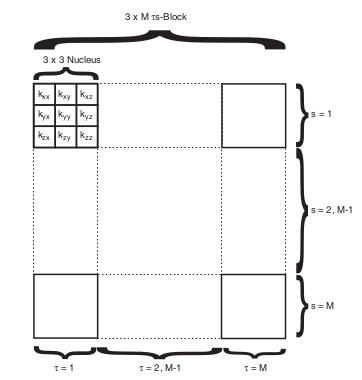
\includegraphics[width=\textwidth]{3.png}
    \caption{Nodal stiffness}
  \end{minipage}
  \hfill
  \begin{minipage}[b]{0.35\textwidth}
    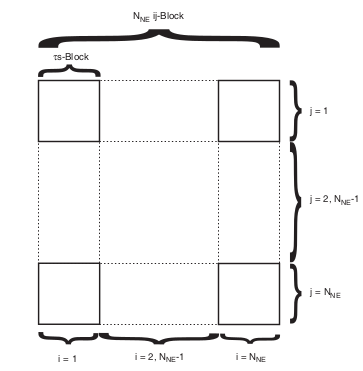
\includegraphics[width=\textwidth]{4.png}
    \caption{Element stiffness}
  \end{minipage}
  \hfill
  \begin{minipage}[b]{0.35\textwidth}
    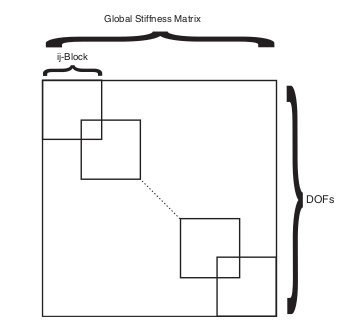
\includegraphics[width=\textwidth]{5.png}
    \caption{Global stiffness}
  \end{minipage}
\end{figure}
The graphical description of the process of assembling stiffness matrix is given in the figure below. 
\begin{figure}[htbp]
\begin{center}
\includegraphics[width=0.7\textwidth]{{6.png}}
 \caption{Graphical description of the FN implementation}
 \label{fig:graph}
\end{center}
\end{figure}
Since L4 Polynomials are used, instead of having single node as if in 1D FEM each node will have four nodal points(beacuse of the L4 expansion). Therefore a single B2(Linear) element has 8 nodes and each node has 3 degree of freedom(DOF). As a result of that each B2 element will have 24*24 element stiffness matrix(8*3). This gets more complex if B3(36*36 matrix) and B4(48*48 matrix) elements are used for the analysis. Therefore appropriate assignment matrix has to be computed for each case in order to assemble the element stiffness matrix to get global stiffness matrix.
\subsubsection*{Load Vector}
\indent\indent\indent The Load Vector for any type of loading can be derived from the equation (4). Let us consider a B2 element having a square cross section is loaded by a downward force P(Z-direction) at the central point of the tip cross section(Cantilever beam). The Load vector is computed by the PVD
\begin{equation}
\delta L_{ext} = F_{\tau}N_{i}P\delta u^{T}_{\tau i}
\label{PVD}
\end{equation}
The value of the shape function at the loading point is 1 and at the fixed end it is zero. Therefore $N_{1} = 0$ and $N_{2} = 1$. P acts in z direction therefore only $u_{z}$ components of the load vector are involved. Therefore the virtual variation of the external work is given by
$$
\delta L_{ext} = P F_{1} u_{z_{11}} + P F_{2} u_{z_{12}} + P F_{3} u_{z_{13}} + P F_{4} u_{z_{14}}
$$
By substituting the value of the natural coordinates($\alpha,\beta$) of the loading position(0,0) in the Lagrange polynomials of the above equation we get
$$
\delta L_{ext} = \frac{P}{4} u_{z_{11}} + \frac{P}{4} u_{z_{12}} + \frac{P}{4} u_{z_{13}} + \frac{P}{4} u_{z_{14}} 
$$
According to the above equation, a load of magnitude $\frac{P}{4}$ has to be placed in the 3,6,9 and 12th postion of the nodal load vector. 

\subsubsection*{Postprocessing (Displacements,Stresses and Strains)}
\indent\indent\indent From the displacement values obtained from the analysis strain and stress values at the point of interest can be obtained. In order to do that the dsiplacement values are expanded over all the points where post processing is needed. This expansion can be done with the help of shape functions. The shape functions $(N_{i}(y))$ along the beam axis and expansion functions $(F_{\tau})$ above the cross section. The equation for expansion is shown in the equation below

\begin{equation}
u_{x}(x_{p},y_{p},z_{p}) = N_{i}(y_{p}) F_{\tau}(x_{p},z_{p})u_{x_{\tau i}}
\end{equation}
\begin{equation}
u_{y}(x_{p},y_{p},z_{p}) = N_{i}(y_{p}) F_{\tau}(x_{p},z_{p})u_{y_{\tau i}}
\end{equation}
\begin{equation}
u_{z}(x_{p},y_{p},z_{p}) = N_{i}(y_{p}) F_{\tau}(x_{p},z_{p})u_{z_{\tau i}}
\end{equation}
where  $[x_{p},y_{p},z_{p}]$ is a generic point of the structure where the displacement values have to be computed. The terms $[u_{x_{\tau i}},u_{y_{\tau i}},u_{z_{\tau i}}]$ are the x,y and z displacment of the nodal points computed from the FE Analysis. 
Stress and strain components are straightforwardly computed from the nodal displacement values. In order to find the strains partial derivatives are required which can be calculated by means of shape and expansion function.

\begin{equation}
u,_{x} = (F_{\tau} N_{i} u_{\tau i}),_{x} = F_{\tau,x} N_{i} u_{\tau i}
\label{u,x}
\end{equation}
\begin{equation}
u,_{y} = (F_{\tau} N_{i} u_{\tau i}),_{y} = F_{\tau} N_{i,y} u_{\tau i}
\label{u,y}
\end{equation}
\begin{equation}
u,_{z} = (F_{\tau} N_{i} u_{\tau i}),_{z} = F_{\tau,z} N_{i} u_{\tau i}
\label{u,z}
\end{equation}
As the strain field is computed, stress components are obtained through the constitutive laws
\begin{equation}
\{\sigma\} = [C]\;\{\epsilon\}
\end{equation}

\section*{Results and Discussion}
\indent\indent\indent\indent Beams subjected to bending loads are analyzed here using Refined 1D beam models. Clamped boundary conditions are accounted for the analysis. The beams are considered to have conventional square cross section and unconventional elliptical cross section. An isotropic material of Young's modulus(E) 75 [Gpa] and a Poisson's ratio of 0.33 is used for both the cases.

\subsection*{Inital Tests}
\indent\indent\indent\indent Before analyzing the above mentioned cross sections, two fundamental test has been conducted in order to test the functionality of the code. The tests are stiffness matrix test and tension test.

\subsubsection*{Stiffness matrix test}
\indent\indent\indent\indent In order to check whether the stiffness matrix derived using the Fundamental Nucleus(FN) technique (a rather new approach) works well, one of the components of the stiffness matrix derived for particular case using analytical solution presented in the literature has been compared with the same component for the same case obtained using the implemented code. The test case is given as follows: A rectangular beam of length L is considered. A B2 element is used along the beam axis and an L4 element is adopted across the cross section. The analytical solution for the 15*3 component of the element stiffness matrix is given below
\begin{equation}
k^{2122}_{xx} = \frac{1}{18} \frac{b L}{a} C_{22} + \frac{1}{18} \frac{a L}{b} C_{66} - \frac{4}{9} \frac{a b}{L} C_{44}
\end{equation}
For a square cross section beam of length L = 2m, cross section of a = b = 0.2m and elastic constants($C_{22},C_{44},C_{66}$) for the above given isotropic material the obtained value of the above component is $1.544*10^{10}$. The value of the same 15*3 component of the element stiffness matrix obtained using the implemented code is $1.522*10^{10}$. This proves that the implemented code complies well with the analytical solution.
\subsubsection*{Tension test}
\indent\indent\indent\indent Since refined 1D beam models are generalized models, tension test can be carried out by deriving appropriate load vector which applies the load in the positive y direction(along beam axis). And also the exact solution for calculating the deformation due to tensile load can be easily derived, it serves as a viable candidate to check whether the displacement obtained from the implemented code is correct or not. The deformation due to tensile load is given by 
\begin{equation}
dL = \frac{P L}{E A}
\label{exactdef}
\end{equation}
where P - load applied, L - length of the beam, A - area of cross section and E - Young's modulus. For a load of 50N and a beam of above given parameters the deformation due to the load P is found to be $3.3*10^{-8}m$. The Load vector for tension load(used in code) can be derived using the equation (\ref{PVD}) by applying the load in positive y direction. The deformation calculated by the implemented code(using 20 B2 elements) due to tensile of 50N is found to be $2.96*10^{-8}$. This proves that the deformation obtained using the implemented model is close enough to the exact solution.
\newpage
\subsection*{Square cross-section beam:}
\indent\indent\indent\indent A cantilever beam of square cross-section undergoing a vertical force, $P_{u_{z}}$, is considered for the analysis. A load ($P_{u_{z}}$) of -50[N] is applied at the central point of the tip cross-section in order to perform typical bending analysis. The sides of the section (a) are equal to 0.2 [m]. The span to height ratio $\frac{L}{h}$ is equal to 10. The mechanics of the beam is described in terms of the maximum vertical displacement($u_{z}$) computed at the central point of the tip cross-section and the maximum absolute value of axial strain and stress. A reference solution for the above given terms is given as follows\\
\\
Maximum vertical displacement 
\begin{equation}
u_{z} = \frac{P_{u_{z}} L^{3}}{3 E I}
\label{u_z}
\end{equation}
\\
Absolute value of maximum strain
\begin{equation}
\epsilon_{yy} = \frac{P_{u_{z}} L h}{2 E I}
\label{eyy}
\end{equation}
\\
Absolute value of maximum stress
\begin{equation}
\sigma_{yy} = \frac{P_{u_{z}} L h}{2 I}
\label{syy}
\end{equation}
\subsubsection*{Maximum vertical displacement ($u_{z}$):}
Tables 4, 5 and 6 presents the maximum vertical displacement, $u_{z}$, computed using Linear (B2), Quadratic (B3) and Cubic (B4) elements respectively along the beam axis. L4 expansion is used across the cross-section for all the cases and a span to height ratio of 10 is used. The reference solution for maximum vertical displacement, $u_{z}$, obtained using the formula (\ref{u_z}) is $-1.333*10^{-5}\;[m]$. From the tables, it is evident that the accuracy of the displacement values increases with increase in number of elements along the beam axis. Because higher number of elements increases the flexibility of the structure. In case of linear elements, the model converges to a maximum displacement of only $-0.9*10^{-5}\;[m]$ as seen from the table (\ref{tab:table 4}).
\begin{table}[h!]
  \begin{center}
     \begin{tabular}{c c}
      \hline\\
      \textbf{No of elements} & \textbf{$u_{z}*10^{5}\;[m]$} \\
      \\
      \hline
      \\[-2pt]
       1 & -0.68 \\[5pt]
       2 & -0.85 \\[5pt]
      10 & -0.90 \\[5pt]
      20 & -0.90 \\[5pt]
      40 & -0.90 \\[5pt]

      \hline
     \end{tabular}
    \caption{Displacement values ($u_{z}$) obtained using B2 element}
    \label{tab:table 4}
  \end{center}
\end{table}
\newpage
The accuracy of the model can be increased by changing the type of element. Table (\ref{tab:table 5}) presents the value of maximum vertical displacement computed using Quadratic element. The model predicts a displacement of $-0.9499*10^{-5}\;[m]$ in the beginning and converges to a maximum displacement of $-1.283*10^{-5}\;[m]$ which is pretty close to the reference solution.
\begin{table}[h!]
  \begin{center}
     \begin{tabular}{c c}
      \hline\\
      \textbf{No of elements} & \textbf{$u_{z}*10^{5}\;[m]$} \\
      \\
      \hline
      \\[-2pt]
       1 & -0.949 \\[5pt]
       2 & -1.224 \\[5pt]
      10 & -1.286 \\[5pt]
      20 & -1.283 \\[5pt]
      40 & -1.283 \\[5pt]

      \hline
     \end{tabular}
    \caption{Displacement values obtained ($u_{z}$) using B3 element}
    \label{tab:table 5}
  \end{center}
\end{table}

Table (\ref{tab:table 6}) presents the maximum vertical displacement obtained using the Cubic element (B4). The model predicts a displacement of $-0.9088*10^{-5}\;[m]$ initally and it stays at the same value even if the number of elements is increased. The cubic element is supposed to be more accurate than quadratic element, on contrary it stays at the same value. The problem could be due to the fact that the cubic element might not work well with L4 polynomial expansion across the cross-section. Therefore, higher order polynomials like L9 or L16 has to be implemented in order to make cubic element models more accurate. 
\begin{table}[h!]
  \begin{center}
     \begin{tabular}{c c}
      \hline\\
      \textbf{No of elements} & \textbf{$u_{z}*10^{5}\;[m]$} \\
      \\
      \hline
      \\[-2pt]
       1 & -0.908 \\[5pt]
       2 & -0.908 \\[5pt]
      10 & -0.908 \\[5pt]
      20 & -0.908 \\[5pt]
      40 & -0.908 \\[5pt]

      \hline
     \end{tabular}
    \caption{Displacement values obtained ($u_{z}$) using B4 element}
    \label{tab:table 6}
  \end{center}
\end{table}

Therefore, it can be concluded that the quadratic beam element has the potential to yield more accurate results provided that L4 polynomial expansion is used across the cross-section. 

\newpage
The comparison of vertical displacements ($u_{z}$) of the central point of the tip cross section for different beam elements is shown in Fig.\ref{fig:Z comparison}. 1, 2, 10, 20, 40 number of elements are considered for the comparison.
\begin{figure}[htbp]
\begin{center}
\includegraphics[width=0.8\textwidth]{{7.png}}
 \caption{$u_{z}$ vs number of beam elements for different type elements}
 \label{fig:Z comparison}
\end{center}
\end{figure}
Fig (\ref{fig:Z_B3}) shows the Z displacement of the central point of all cross-sections of the beam. It shows the typical bending behaviour of the beam. The displacements are computed using 20 B3 elements along the beam axis and L4 polynomials across the cross-section. 
\\
\\
\begin{figure}[htbp]
\begin{center}
\includegraphics[width=0.53\textwidth]{{8.png}}
 \caption{Displacement ($u_{z}$) of the beam using 20 B3 elements }
 \label{fig:Z_B3}
\end{center}
\end{figure}
\newpage
\subsubsection*{Maximum axial strain and stress ($\epsilon_{yy}$, $\sigma_{yy}$):}
\indent\indent\indent\indent  The main aim of the refined 1D beam model is to predict the 3D behaviour of the beam when subjected to loading. With the help of X, Y and Z displacements, strains and stresses at any point in the beam can be computed using the equations \ref{u,x}, \ref{u,y} and \ref{u,z}. Since vertical load is applied in the beam, X displacement becomes zero so it can be neglected. The maximum axial strain and stress given by the equations \ref{eyy} and \ref{syy} serves as a reference solution for comparing the stresses and strains computed by our model. Since maximum axial strains and stresses are present in the fixed end, it can be computed with the help of Y displacements of the section close to the fixed end. With the help of displacements, shape functions and equation \ref{u,y}, axial strain ($\epsilon_{yy}$) at any point in the cross-section can be computed. Fig \ref{fig:eyy}, presents the variation of axial strain above the cross-section at the fixed end computed using 40 B4 elements along the beam axis and a 50*50 meshgrid.
\\
\\
\begin{figure}[htbp]
\begin{center}
\includegraphics[width=0.7\textwidth]{{9.png}}
 \caption{Axial strain ($\epsilon_{yy}$) above the cross-section at y=0}
 \label{fig:eyy}
\end{center}
\end{figure}

Table \ref{tab:table 7} presents the absolute value and the position of maximum axial strains and stresses computed at the fixed end (Y=0) using different type of elements. The position of maximum stresses and strains does not depend on x. It is observed from the table that maximum stress and strain computed using B2 and B3 elements agrees well with the reference soltion. But the values computed using B4 element does not matches well because of the fact that B4 element requires higher order expansion across the cross-section to increase its accuracy. Fig \ref{fig:eyy_y} and  \ref{fig:syy_y} presents the variation in the axial strain and stress versus z at x = y = 0.

\newpage
\begin{table}[h!]
  \begin{center}
     \begin{tabular}{c c c p{2cm} c c}
      \hline\\
      \textbf{Type of element} & \textbf{$\epsilon_{zz}*10^{6}$} & \textbf{$\sigma_{zz}\;[MPa]$} &                    \textbf{x} & \textbf{y} & \textbf{z} \\
      \\
      \hline
      \\[-2pt]
       Ref soln & 1.000  & 0.075 & $-\frac{b}{2} \leq +\frac{b}{2}$ & $\pm \frac{h}{2}$ & 0 \\[5pt]
       B2       & 1.333 &  0.099 & $-\frac{b}{2} \leq +\frac{b}{2}$ & $\pm \frac{h}{2}$ & 0 \\[5pt]
       B3       & 1.333 &  0.099 & $-\frac{b}{2} \leq +\frac{b}{2}$ & $\pm \frac{h}{2}$ & 0 \\[5pt]
       B4       & 0.448 &  0.033 & $-\frac{b}{2} \leq +\frac{b}{2}$ & $\pm \frac{h}{2}$ & 0 \\[5pt]
     
      \hline
     \end{tabular}
    \caption{Displacement values obtained ($u_{z}$) using B4 element (40 elements)}
    \label{tab:table 7}
  \end{center}
\end{table}



From fig \ref{fig:eyy_y}, it is observed that B2 and B3 beam elements produces almost same strain values and they are close to the reference solution. But the values computed by B4 element is not close to the reference solution. The same can be observed for the fig \ref{fig:syy_y} which shows the axial stress vs y at x = y = 0.  
\\
\\
\begin{figure}[htbp]
\begin{center}
\includegraphics[width=0.73\textwidth]{{10.png}}
 \caption{Axial strain ($\epsilon_{yy}$) vs z at x=0 and y=0. Type of  element:B4. 40 beam elements.}
 \label{fig:eyy_y}
\end{center}
\end{figure}

With the maximum stress and strain verified using the reference solution, the distribution of strains and stresses at any point in the beam can be found out using the displacement values obtained at the nodes and shape functions. Figure \ref{fig:strain_dis} and \ref{fig:stress_dis} shows the distribution of strains and stresses at the cross-section close to the fixed end.
\newpage
\begin{figure}[htbp]
\begin{center}
\includegraphics[width=0.7\textwidth]{{11.png}}
 \caption{Axial stress ($\sigma_{yy}$) vs z at x=0 and y=0. Type of  element:B4. 40 beam elements.}
 \label{fig:syy_y}
\end{center}
\end{figure} 
This distribution of strains and stresses are obtained by computing strain values at all the points in a 50*50 meshgrid by interpolation of strains with the help of displacements and shape functions.
\\
\\ 
\begin{figure}[H]
\begin{center}
\includegraphics[width=0.7\textwidth]{{12.png}}
 \caption{Distribution of strain at the fixed end cross-section ($\epsilon_{yy}$)}
 \label{fig:strain_dis}
\end{center}
\end{figure}

\newpage
\begin{figure}[H]
\begin{center}
\includegraphics[width=0.7\textwidth]{{13.png}}
 \caption{Distribution of stress at the fixed end cross-section ($\sigma_{yy}$)}
 \label{fig:stress_dis}
\end{center}
\end{figure}

In order to check whether the implemented model can be applied for practical applications, a NASTRAN model has been built for the comparison purpose. Fig \ref{fig:nastran} presents the NASTRAN model which shows the distribution of axial stress ($\sigma_{yy}$). It is observed from the figure that it shows a stress range of -0.0905 [MPa] to 0.0916 [MPa]. This close enough to our implemented model where the stress ranges from -0.1 [MPa] to 0.1 [MPa] as seen in the figure \ref{fig:stress_dis}.
\\
\\
\\
\begin{figure}[H]
\begin{center}
\includegraphics[width=0.7\textwidth]{{14.png}}
 \caption{NASTRAN model showing the distribution of axial stress ($\sigma_{yy}$) }
 \label{fig:nastran}
\end{center}
\end{figure}
\newpage
\subsubsection*{Y displacement of the tip cross-section:}
\indent\indent\indent\indent Y displacement of the tip cross-section gives a better understanding of the tilt of the end cross-section visually which cannot be obtained from classical beam models like Euler-Bernoulli. Y displacement of the nodes of end cross-section and shape functions are used to interpolate the displacement values across the whole cross-section using 50*50 meshgrid. 
\\
\\
\\
\begin{figure}[!htbp]
  \centering
  \begin{minipage}[b]{0.45\textwidth}
    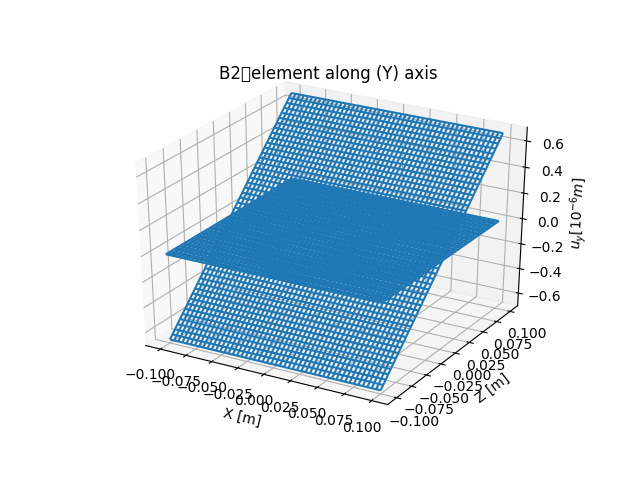
\includegraphics[width=\textwidth]{15.png}
    \caption{B2 element along Y axis}
    \label{fig: Y_B2}
  \end{minipage}
  \hfill
  \begin{minipage}[b]{0.45\textwidth}
    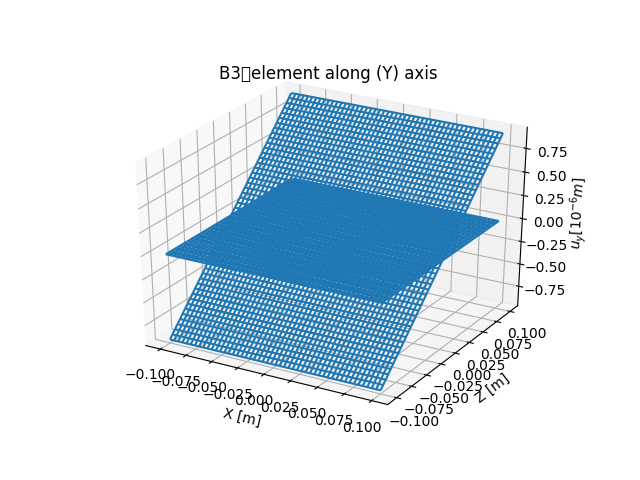
\includegraphics[width=\textwidth]{16.png}
    \caption{B3 element along Y axis}
    \label{fig: Y_B3}
  \end{minipage}
  \hfill
  \begin{minipage}[b]{0.45\textwidth}
    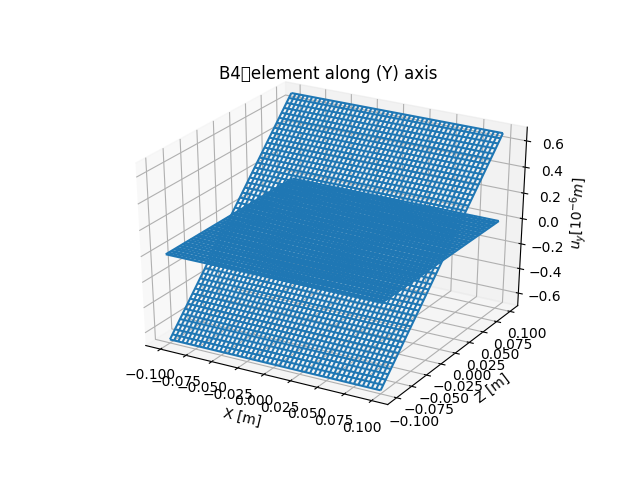
\includegraphics[width=\textwidth]{17.png}
    \caption{B4 element along Y axis}
    \label{fig: Y_B4}
  \end{minipage}
\end{figure}

Figure \ref{fig: Y_B2}, \ref{fig: Y_B3} and \ref{fig: Y_B4} shows the tilt of end cross-section computed using 40 B2, B3 an B4 elements respectively. Table \ref{tab:table 8}  shows the comparison of peak Y displacements computed using our implemented model and the NASTRAN model. It is observed from the table that the accuracy of the solution increases with changing the type of element and the displacement computed using B3 element is pretty much close to the NASTRAN model. Since the B4 element does not work well with the L4 polynomial the maximum displacement obtained is same as that of B4 element.
\newpage
\begin{table}[h!]
  \begin{center}
     \begin{tabular}{c c}
      \hline\\
      \textbf{Element type} & \textbf{$u_{y}*10^{7}\;[m]$} \\
      \\
      \hline
      \\[-2pt]
       NASTRAN sol. & 9.99 \\[5pt]
       B2 & 6.74\\[5pt]
       B3 & 9.31 \\[5pt]
       B4 & 6.74 \\[5pt]

      \hline
     \end{tabular}
    \caption{Displacement ($u_{y}$) computed  using type of elements. No of elements 40.}
    \label{tab:table 8}
  \end{center}
\end{table}
\subsection*{Elliptical Cross-section:}
\indent\indent\indent\indent Refined 1D beam model can be extended to any beam structures of arbitrary cross-section with the help of expansion functions across the cross-section. In order to check the ubiquity of our model an elliptical cross-section has been chosen. Clamped boundary conditions are accounted for the analysis. The length of the beam is 4[m] and the major and minor axis are 0.8 and 0.4[m] respectively. A vertical force ($P_{u_{z}}$) of -100[N] is applied at the central point of the tip cross-section. The elliptical cross-section is modeled by fitting a maximum possible rectangle inside the ellipse and analysed using appropriate jacobian value. Since we have no reference solution for elliptical cross-section beam a NASTRAN model has been built for the comparison purposes. The table \ref{tab:table 9} below shows the comparison of maximum vertical displacement of the NASTRAN model and the model built using different type of elements(For 40 elements). It is observed from the table that the model behaves as same for square cross-section. The accuracy of the model is high with the B3 element and the maximum displacement of the B4 element is same as that of B2.
\\
\begin{table}[h!]
  \begin{center}
     \begin{tabular}{c c}
      \hline\\
      \textbf{Element type} & \textbf{$u_{z}*10^{7}\;[m]$} \\
      \\
      \hline
      \\[-2pt]
       NASTRAN sol. & -7.08 \\[5pt]
       B2 & -5.84\\[5pt]
       B3 & -8.01 \\[5pt]
       B4 & -5.84 \\[5pt]

      \hline
     \end{tabular}
    \caption{Displacement ($u_{z}$) computed  using type of elements. No of elements 40.}
    \label{tab:table 9}
  \end{center}
\end{table}

Figure \ref{fig:ell_uz} presents the Z displacement of the central point of all cross-sections computed using 40 B3 elements which shows the bending behaviour of the beam.
\newpage
\begin{figure}[H]
\begin{center}
\includegraphics[width=0.7\textwidth]{{18.png}}
 \caption{Dislacement ($u_{z}$) computed using 40 B3 elements  }
 \label{fig:ell_uz}
\end{center}
\end{figure}

Y displacement of the tip cross-section helps us to visualize the tilt of the beam cross-section. The cross-section here is constructed with a 100*100 mesh grid of side length equal to the major axis and then excluding the grid points which are not in the ellipse with the help of the equation of the ellipse. The formula \ref{ellipse} shows the equation of the ellipse
\\
\begin{equation}
\frac{x^{2}}{a^{2}} + \frac{y^{2}}{b^{2}} = 1
\label{ellipse}
\end{equation}

where x and y are the coordinate points and a and b are the semi- major and semi-minor axis respectively. The table \ref{tab:table 10}  shows the comparison of peak Y displacement of the NASTRAN model and the our model computed using different type of elements. It is seen that the model behaves as same as that of square cross-section where B3 is more accurate and B2 and B4 are same.
\\
\begin{table}[h!]
  \begin{center}
     \begin{tabular}{c c}
      \hline\\
      \textbf{Element type} & \textbf{$u_{y}*10^{7}\;[m]$} \\
      \\
      \hline
      \\[-2pt]
       NASTRAN sol. & 1.05 \\[5pt]
       B2 & 0.84\\[5pt]
       B3 & 1.15 \\[5pt]
       B4 & 0.84 \\[5pt]

      \hline
     \end{tabular}
    \caption{Peak displacement ($u_{y}$) computed  using type of elements. No of elements 40.}
    \label{tab:table 10}
  \end{center}
\end{table}


Fig \ref{fig: Y_B2_ell}, \ref{fig: Y_B3_ell} and \ref{fig: Y_B4_ell} presents the y displacement of the end cross-section which gives a visualization of how the beam cross-section tilts when loaded with a vertical force of -100 [N].
\\
\\ 
\\
\begin{figure}[!htbp]
  \centering
  \begin{minipage}[b]{0.49\textwidth}
    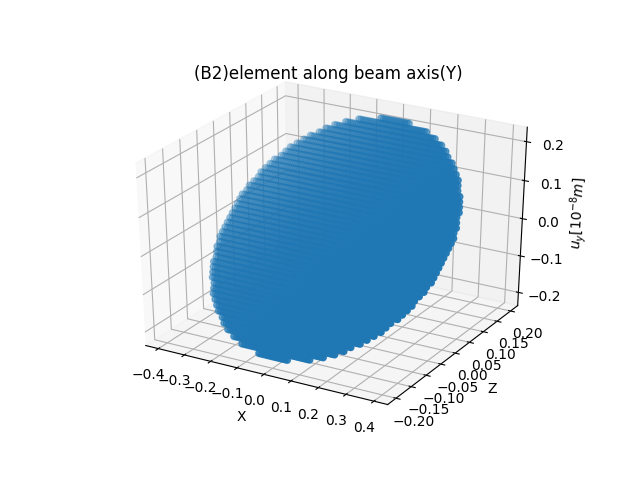
\includegraphics[width=\textwidth]{19.png}
    \caption{B2 element along Y axis}
    \label{fig: Y_B2_ell}
  \end{minipage}
  \hfill
  \begin{minipage}[b]{0.49\textwidth}
    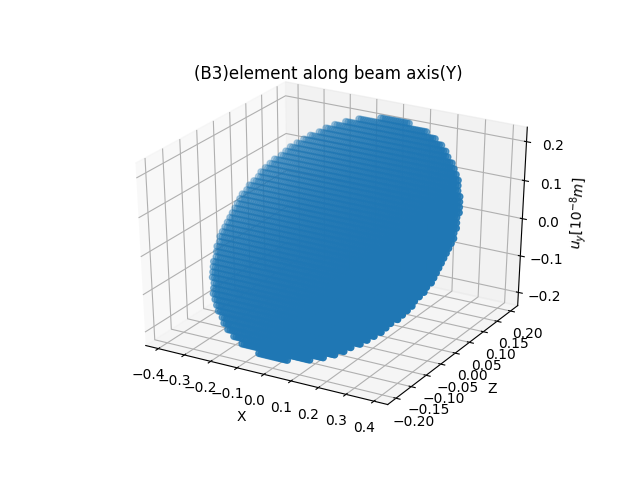
\includegraphics[width=\textwidth]{20.png}
    \caption{B3 element along Y axis}
    \label{fig: Y_B3_ell}
  \end{minipage}
  \hfill
  \begin{minipage}[b]{0.49\textwidth}
    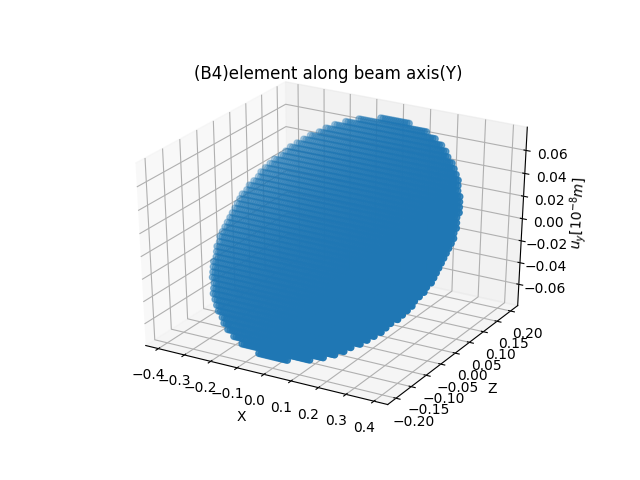
\includegraphics[width=\textwidth]{21.png}
    \caption{B4 element along Y axis}
    \label{fig: Y_B4_ell}
  \end{minipage}
\end{figure}

The distribution of strains and stresses are obtained by computing strain values at all the points in a 50*50 meshgrid by interpolation of strains with the help of displacements and shape functions. Figure \ref{fig:strain_dis_ell} and \ref{fig:stress_dis_ell} shows the distribution of the strains ($\epsilon_{yy}$)  and  axial stresses ($\sigma_{yy}$)  at the cross-section close to the fixed end because this is the area of maximum strains and stresses.\\ 
\\
In order to check the accuracy of our model, the maximum stress obtained is compared with the NASTRAN model. The maximum stress range obtained from the NASTRAN model ranges from -0.059 [MPa] to 0.055 [Mpa] which is close to our model which has a stress range of -0.033 [MPa] to 0.033 [MPa].

\begin{figure}[H]
\begin{center}
\includegraphics[width=0.7\textwidth]{{22.png}}
 \caption{Distribution of axial strain at the fixed end cross-section ($\epsilon_{yy}$)}
 \label{fig:strain_dis_ell}
\end{center}
\end{figure}


\begin{figure}[H]
\begin{center}
\includegraphics[width=0.7\textwidth]{{23.png}}
 \caption{Distribution of axial stress at the fixed end cross-section ($\sigma_{yy}$)}
 \label{fig:stress_dis_ell}
\end{center}
\end{figure}


Figure \ref{fig:nastran_ell}  given below presents an elliptical beam model built using NASTRAN. It shows the range of maximum axial stress ($\sigma_{yy}$) at the cross-secction close to the fixed end when subjected to a vertical load ($P_{u_{z}}$) of -100[N]. 

\begin{figure}[H]
\begin{center}
\includegraphics[width=0.7\textwidth]{{24.png}}
 \caption{NASTRAN model showing the distribution of axial stress ($\sigma_{yy}$) }
 \label{fig:nastran_ell}
\end{center}
\end{figure}



\end{document}

